\documentclass[11pt,a4paper]{article}

\usepackage{amsmath}
\usepackage{authblk}
\usepackage[british]{babel}
\usepackage[backend=biber, style=authoryear]{biblatex}
\usepackage{csquotes}
\usepackage{graphicx}
\usepackage{hyperref}
\usepackage[T1]{fontenc}

\hypersetup{
  colorlinks=true,
  urlcolor=blue,
  linkcolor=black,
  citecolor=black
}

\addbibresource{ev_wake_model_implementation.bib}

\title{Implementation of the Eddy Viscosity (EV) wake model in PyWake}

\author{Christian Jonsson}
\author{Alistair Merry}
\affil{The Natural Power Consultants Limited}

\date{\today}

\begin{document}

\maketitle

\begin{abstract}
This paper describes an implementation of the Eddy Viscosity (EV) wind turbine wake model in the PyWake software package. It outlines the system of governing equations and discussed the computational approach to the solution along with integration in the PyWake framework.
\end{abstract}

\renewcommand\abstractname{Disclaimer}
\begin{abstract}
The Natural Power Consultants Limited accepts no liability whatsoever in connection with this paper or any software tools that make use of material presented here. Any use of this material is at the sole risk of the user.
\end{abstract}

\section{Introduction}\label{introduction}

The Eddy Viscosity (EV) wind turbine wake model developed by \textcite{Ainslie_1988} is widely used in the wind energy industry for pre-construction energy yield assessments (EYAs), sometimes with various modifications and extensions. It is implemented in many industry-standard EYA modelling tools, such as WindFarmer and Openwind. This paper describes the implementation of this model in the \href{https://gitlab.windenergy.dtu.dk/TOPFARM/PyWake}{PyWake} software package published by DTU.

PyWake provides a flexible and powerful framework for executing computations in an automated fashion and comparing results from different models. The motivation for implementing the EV model in PyWake is to allow for more convenient execution of wake loss calculations with this model, replication of legacy wake computations that rely on this model and inclusion of this model in benchmarking exercises.

\textcite{Anderson_2011} developed a simplified solution to the EV model equations by observing that the wake profile is self-similar in the streamwise direction. His approach allows for a reduction of the system of governing equations from two dimensions (steam-wise and radial distance from the wind turbine rotor centre) to one dimension (streamwise distance only), making them considerably easier and faster to solve. Because this simplification sacrifices neither accuracy nor precision of the solution to any material extent, it appears the obvious choice of approach and has been adopted in the EV model implementation in PyWake.

The remainder of this paper is structured as follows. The formulation of the system of equations, with possible variations, is described in §\ref{formulation}. The computational approach to the solution is outlined in §\ref{computational_approach} and integration in the PyWake framework is discussed in §\ref{pywake_integration}. Finally a basic comparison of results against those presented by \textcite{Anderson_2011} and calculated using the industry-standard tools WindFarmer and Openwind is provided in §\ref{results_comparison}.

\section{Formulation}\label{formulation}

\subsection{Simplified formulation for centreline wake velocity}\label{wake_velocity_formulation}

\textcite{Anderson_2011} provided the following\footnote{Note that the notation used here is somewhat different from that of \textcite{Anderson_2011}.} simplified formulation of the governing equations of fluid motion in the wake of a single wind turbine:
\begin{equation}\label{eq:gov_uc}
\frac{\textrm{d}\tilde{u}_{c}}{\textrm{d}\tilde{x}} =
  \frac{16 \, \tilde{\epsilon} \left( \tilde{u}_{c}^{3} - \tilde{u}_{c}^{2} - \tilde{u}_{c} + 1 \right)}{C_{t} \, \tilde{u}_{c}},
\end{equation}
where $\tilde{u}_{c}$ is the dimensionless streamwise component of the wind centreline velocity in the wake, $\tilde{x}$ the non-dimensional downwind distance from the rotor, $C_{t}$ the wind turbine thrust coefficient and $\tilde{\epsilon}$ the non-dimensional wake eddy viscosity.

The non-dimensional quantities $\tilde{u}_{c}$ and $\tilde{x}$ are defined as
\begin{equation}
\begin{array}{ l l l }
  \tilde{u}_{c} & = & \frac{u_{c}}{U_{0}} \textrm{; and} \\
  \tilde{x}     & = & \frac{x}{D},
\end{array}
\end{equation}
where $u_{c}$ is the dimensional streamwise wake centreline wind speed, $U_{0}$ the free-stream (undisturbed incident) wind speed, $x$ the dimensional downtime distance from the rotor and $D$ the diameter of the wind turbine rotor.

The thrust coefficient is defined as
\begin{equation}
C_{t} = \frac{F_{t}}{\frac{1}{2} \rho A \, U_{0}^{2}}
\end{equation}
where $F_{t}$ is the streamwise thrust force on the rotor, $\rho$ the air density and $A = \pi (\frac{D}{2})^{2}$ the rotor swept area. It is noted that $F_{t}$ varies with $U_{0}$ and depends on the wind turbine control. Typically $C_{t}$ specifications are provided by a wind turbine OEM as tabulated binned values as a function of $U_{0}$, together with the power curve specification.

The non-dimensional wake eddy viscosity is a function of $\tilde{u}_{c}$ and $\tilde{x}$, defined as\footnote{Combining different equations given by \textcite{Anderson_2011}.}
\begin{equation}\label{eq:epsilon_uc}
\tilde{\epsilon} (\tilde{x}, \tilde{u}_{c}) =
  F(\tilde{x}) \left(
    0.015 \left( \sqrt{\frac{3.56 C_{t}}{4 \left( 1 - \tilde{u}_{c}^{2} \right)}} \right) \left( 1 - \tilde{u}_{c} \right)+ 0.16 I_{0}
  \right)
\end{equation}
where $I_{0}$ is the ambient (upstream) turbulence intensity\footnote{Note that \textcite{Ainslie_1988} and \textcite{Anderson_2011} define $I_{0}$ as a percentage value and the definition here uses the unscaled standard non-dimensional quantity. Hence there is a difference of a factor of 100.} and $F(x)$ a filter function to adjust for near-wake mixing.

\textcite{Ainslie_1988} defined the filter function as follows (also used in the formulation by \cite{Anderson_2011}):
\begin{equation}\label{eq:filter_function}
F(\tilde{x}) = \left\{
  \begin{array}{ l l }
    0.65 + \left( \frac{\tilde{x} - 4.5}{23.32} \right) ^{\frac{1}{3}} & \quad \textrm{if } \tilde{x} < 5.5 \textrm{, and} \\
    1.0                                                                & \quad \textrm{if } \tilde{x} \geq 5.5.
  \end{array}
\right.
\end{equation}

The WindFarmer Theory Manual \parencite{WindFarmer_Theory_Manual} explains that $F$ is fixed at unity in the WindFarmer implementation of the EV model based on validation against measurements reported by \textcite{Taylor_1990}. In Openwind \parencite{Openwind_Theory_Manual}, the near wake mixing filter function can be enabled or disabled by the user, where the default setting is keeping it enabled.

The governing differential equation (\ref{eq:gov_uc}) expresses the downwind rate of change of $\tilde{u}_{c}$ with downwind distance $\tilde{x}$ as a function of the values of $\tilde{u}_{c}$ and $\tilde{x}$. Given an initial value, it can be solved for downwind. \textcite{Ainslie_1988} proposed adopting the following initial value, which was also used by \textcite{Anderson_2011}:
\begin{equation}\label{eq:initial_uc}
\tilde{u}_{c} (\tilde{x} = 2) = 1 - C_{t} + 0.05 + (16 C_{t} - 0.5) \left( \frac{I_{0}}{10} \right).
\end{equation}

In the near wake, for values of $\tilde{x}$ less than 2, $\tilde{u}_{c}$ is not defined. The EV model is not applicable in the near wake as it does not account for pressure gradients, which play an important role in the flow near to the rotor.

\subsection{Simplified formulation for centreline wake deficit}\label{wake_deficit_formulation}

The formulation of the system of equations for the wake centreline velocity in §\ref{wake_velocity_formulation} can be rearranged in terms of the velocity deficit. This is a somewhat more convenient form to work with and fits more directly in the PyWake framework, since a PyWake wake deficit model is expected to provide wind speed deficit values rather than wind speed values. The non-dimensional centreline wake velocity deficit, $\tilde{u}_{d_{c}}$, is governed by the following equation:

\begin{equation}\label{eq:gov_ud}
\frac{\textrm{d}\tilde{u}_{d_{c}}}{\textrm{d}\tilde{x}} =
  \frac{-16 \, \tilde{\epsilon} \, \tilde{u}_{d_{c}}^{2} \left( 2 - \tilde{u}_{d_{c}} \right)}{C_{t} \left( 1 - \tilde{u}_{d_{c}} \right)}.
\end{equation}

The eddy viscosity function can be expressed as:
\begin{equation}\label{eq:epsilon_ud}
\tilde{\epsilon} (\tilde{x}, \tilde{u}_{d_{c}}) =
  F(\tilde{x}) \left(
    0.015 \, \tilde{u}_{d_{c}} \left( \sqrt{\frac{3.56 C_{t}}{4 \, \tilde{u}_{d_{c}} \left( 2 - \tilde{u}_{d_{c}} \right)}} \right) + 0.16 I_{0}.
  \right)
\end{equation}

When expressed in terms of $\tilde{u}_{d_{c}}$, the equation for the initial value becomes
\begin{equation}\label{eq:initial_ud}
\tilde{u}_{d_{c}} (\tilde{x} = 2) = C_{t} - 0.05 - (16 C_{t} - 0.5) \left( \frac{I_{0}}{10} \right).
\end{equation}

\subsection{Wake width}\label{wake_width}

The wake deficit profile is assumed to take a Gaussian form \parencite{Ainslie_1988, Anderson_2011}:
\begin{equation}\label{eq:wake_deficit_profile}
\tilde{u}_{d} (\tilde{x}, \tilde{r}) = \tilde{u}_{d_{c}} (\tilde{x}) \, \exp \left( -3.56 \left( \frac{\tilde{r}}{\tilde{w}} \right)^{2} \right),
\end{equation}
where $\tilde{r} = \frac{r}{D}$ is the non-dimensional radial distance from the wake centreline and $\tilde{w} = \frac{w}{D}$ is the non-dimensional wake width, defined as an estimate of the full width of the wake.

From conservation of momentum, $\tilde{w}$ can be expressed as \parencite{Ainslie_1988, Anderson_2011}:
\begin{equation}\label{eq:wake_width}
\tilde{w} = \sqrt{\frac{3.56 C_{t}}{4 \, \tilde{u}_{d_{c}} \left( 2 - \tilde{u}_{d_{c}} \right)}}.
\end{equation}

\subsection{Wake turbulence model}\label{wake_turbulence_model}

The EV wake deficit model is often implemented in conjunction with the wake added turbulence model proposed by \textcite{QuartonAndAinslie1990}. Both the WindFarmer and Openwind implementations uses a version of this wake turbulence model to adjust the incident turbulence intensity input to the EV model to account for added turbulence from the wakes of upstream turbines (i.e. for turbines not in the free wind stream).

The original empirical formulation proposed by \textcite{QuartonAndAinslie1990} provides the following equation for the added turbulence:
\begin{equation}\label{eq:added_turbulence_original}
I_{+} = 4.8 \, C_{t}^{0.7} \, I_{0}^{0.68} \left( \frac{x}{x_{n}} \right)^{-0.57},
\end{equation}
where $I_{+}$ is the wake added turbulence intensity estimate, $x_{n}$ is an estimate of the near wake length and the other terms are as defined previously.

\textcite{Hassan1992} proposed the following modified empirical formulation based on new experimental data:
\begin{equation}\label{eq:added_turbulence_modified}
I_{+} = 5.7 \, C_{t}^{0.7} \, I_{0}^{0.68} \left( \frac{x}{x_{n}} \right)^{-0.96}.
\end{equation}

The PyWake implementation includes both variations, with the modified formulation used as default. Both WindFarmer and Openwind use the modified formulation.

The estimate of the near wake length $x_{n}$ is based upon an empirical calculation method proposed by Vermeulen and colleagues \parencite{Vermeulen1980, VermeulenAndBuiltjes1981, VermeulenAndVijge1981}, which can be expressed as
\begin{equation}\label{eq:near_wake_length}
x_{n} = \frac{n \, r_{0}}{\frac{\textrm{d}r}{\textrm{d}x}}.
\end{equation}
The parameter $n$ is calculated as
\begin{equation}\label{eq:near_wake_length_n}
n = \frac{n_{1} \left( 1 - n_{2} \right)}{n_{2} \left( 1 - n_{1} \right)}, \enspace
n_{1} = \sqrt{0.214 + 0.144 \, m}, \enspace
n_{2} = \sqrt{0.134 + 0.124 \, m},
\end{equation}
where
\begin{equation}\label{eq:near_wake_length_m}
m = \frac{1}{\sqrt{1 - C_{t}}}.
\end{equation}
The parameter $r_{0}$ is calculated as
\begin{equation}\label{eq:near_wake_length_r0}
r_{0} = \frac{D}{2} \sqrt{\frac{m + 1}{2}}.
\end{equation}
The wake growth rate $\frac{\textrm{d}r}{\textrm{d}x}$ is calculated as
\begin{equation}\label{eq:near_wake_length_drdx}
\frac{\textrm{d}r}{\textrm{d}x} = \sqrt{\left(\frac{\textrm{d}r}{\textrm{d}x}\right)_{\alpha}^2 + \left(\frac{\textrm{d}r}{\textrm{d}x}\right)_{m}^2 + \left(\frac{\textrm{d}r}{\textrm{d}x}\right)_{\lambda}^2},
\end{equation}
where the term $\left(\frac{\textrm{d}r}{\textrm{d}x}\right)_{\alpha}$ is the contribution from ambient turbulence and calculated as
\begin{equation}\label{eq:near_wake_length_drdx_alpha}
\left(\frac{\textrm{d}r}{\textrm{d}x}\right)_{\alpha} = 2.5 \, I_{0} + 0.005,
\end{equation}
the term $\left(\frac{\textrm{d}r}{\textrm{d}x}\right)_{m}$ is the contribution from turbulence generated by shear forces and calculated as
\begin{equation}\label{eq:near_wake_length_drdx_m}
\left(\frac{\textrm{d}r}{\textrm{d}x}\right)_{m} = \frac{\left(1 - m\right) \sqrt{1.49 + m}}{9.76 \left(1 + m\right)}
\end{equation}
the term $\left(\frac{\textrm{d}r}{\textrm{d}x}\right)_{\lambda}$ is the contribution from mechanical turbulence calculated as
\begin{equation}\label{eq:near_wake_length_drdx_lambda}
\left(\frac{\textrm{d}r}{\textrm{d}x}\right)_{\lambda} = 0.012 \, B \, \lambda,
\end{equation}
where $B$ is the number of rotor blades and $\lambda$ is the tip speed ratio.

The wake added turbulence intensity calculated by this model provides an estimate of additional turbulence intensity relative to the freestream wind speed. For values relative to the reduced wind speed in the wake, the results need to be re-normalised relative to the waked wind speed.

\section{Computational approach}\label{computational_approach}

Considering the wake centreline deficit formulation, equations \ref{eq:gov_ud}, \ref{eq:epsilon_ud} and \ref{eq:filter_function} can be combined into a single differential equation where $\frac{\textrm{d}}{\textrm{d}\tilde{x}}(\tilde{u}_{d_{c}})$ is a function of $\tilde{u}_{d_{c}}$, $\tilde{x}$, $C_{t}$ and $I_{0}$. For given values of $C_{t}$ and $I_{0}$, the initial value problem can be solved over the range of relevant downwind distances ($\tilde{x}$), starting at the initial $\tilde{u}_{d_{c}}$ value calculated from equation \ref{eq:initial_ud}. Thus a three dimensional array of $\tilde{u}_{d_{c}}$ can be pre-computed over relevant coordinates along the dimensions $\tilde{x}$, $C_{t}$ and $I_{0}$.

The same approach can of course also be taken for the original wake centreline wind speed formulation. The PyWake implementation includes both the wind speed formulation in §\ref{wake_velocity_formulation} and the deficit formulation in §\ref{wake_deficit_formulation}. The results (lookup tables) arrived at from using the two alternative formulations were found to be very close.

The use of a pre-computed lookup tables is more efficient than solving the initial value problem for each individual case in a model run, since the number of cases is large for realistic scenarios. A vectorised solver could readily be built with the \href{https://docs.scipy.org/doc/scipy/reference/generated/scipy.integrate.solve_ivp.html}{SciPy IVP solver}, using the explicit Runge-Kutta method "RK45".

For each value $\tilde{u}_{d_{c}}(\tilde{x}, C_{t}, I_{0})$, a corresponding value $\tilde{w}(\tilde{x}, C_{t}, I_{0})$ can be computed from equation \ref{eq:wake_width}. Hence a three-dimensional array of $\tilde{w}$ with the same coordinates as the array for $\tilde{u}_{d_{c}}$ can be derived.

From the pre-computed arrays of $\tilde{u}_{d_{c}}$ and $\tilde{w}$, $\tilde{u}_{d}(\tilde{x}, \tilde{r}, C_{t}, I_{0})$ can readily be calculated from equation \ref{eq:wake_deficit_profile}.

\section{PyWake integration}\label{pywake_integration}

\subsection{Vectorised calculations}\label{vectorised_calculations}

The PyWake computational framework uses vectorised calculations along the following dimensions:
\begin{equation}\label{eq:pywake_indices}
\begin{array}{ l l }
  i: & \textrm{source turbine;}\\
  j: & \textrm{downwind turbine or other point;}\\
  k: & \textrm{reference wind speed; and}\\
  l: & \textrm{reference wind direction.}
\end{array}
\end{equation}

The EV wake model equations have been vectorised to compute matrices (arrays) of velocity deficit, wake width and added turbulence as a function of matrices of the required input data, including local free and waked wind speeds, local turbulence intensity, turbine downwind and crosswind spacings, rotor diameters and thrust coefficients.

\subsection{Rotor averaging and wake superposition}\label{rotor_averaging_and_wake_superposition}

The integration of the EV wake model into the PyWake framework only required implementing the new single wake models. The models to account for variations across the rotor and to combine multiple wake effects could be adopted from existing implementation.

As a default, the EV deficit model has been implemented to use a grid rotor average model, thus estimating the effective wind speed of a waked turbine as an average of the predictions across the rotor.

The added turbulence model has been implemented under the assumption that the additional turbulence is constant across the wake. Using the wake width as an approximate measure of the limit to the region where the turbulence is elevated, an area overlap model has been used to weight the prediction by the proportion of a target turbine rotor that is within the limits of the wake from a source turbine.

The usual method for combining wake deficit estimates from multiple turbines with the EV model is to take the largest deficit rather than to let multiple deficits accumulate. The maximum is then taken is taken for each wind speed and wind direction bin. This approach has been adopted as the default implementation in the PyWake EV model. Accordingly, the wake wind speeds are scaled with the free wind speed values rather than with the effective (wake-affected) wind speeds.

The effective incident turbulence intensity is calculated as the root sum square of the ambient turbulence intensity and the estimated maximum wake added turbulence intensity (the estimate from the single turbine with the largest contribution). As noted in §\ref{wake_turbulence_model}, the estimated value is subsequently scaled to correspond to the reduced wind speed in the wake.

The approaches taken in the PyWake implementation are broadly in line with the WindFarmer and Openwind implementations, though not necessarily in all the detail.

\section{Comparison of results}\label{results_comparison}

As a validation of the solver and lookup table generator, a comparison of single wake centreline deficit results was made against the cases presented by \textcite{Anderson_2011}. Results calculated using the Openwind software were also included for reference, both using the standard EV model in the latest version and using the 'FastEddy' implementation of the simplified solution in the older Community Edition (CE) version. A plot showing the different results, which are all in good agreement, is presented in Figure \ref{fig:wake_recovery_results_comparison_mixing_function}. In all of these results, the near wake mixing filter function is enabled. WindFarmer results are not included for this case, since WindFarmer always has the near wake mixing filter function disabled (i.e. it is not configurable).

\begin{figure}
	\centering
		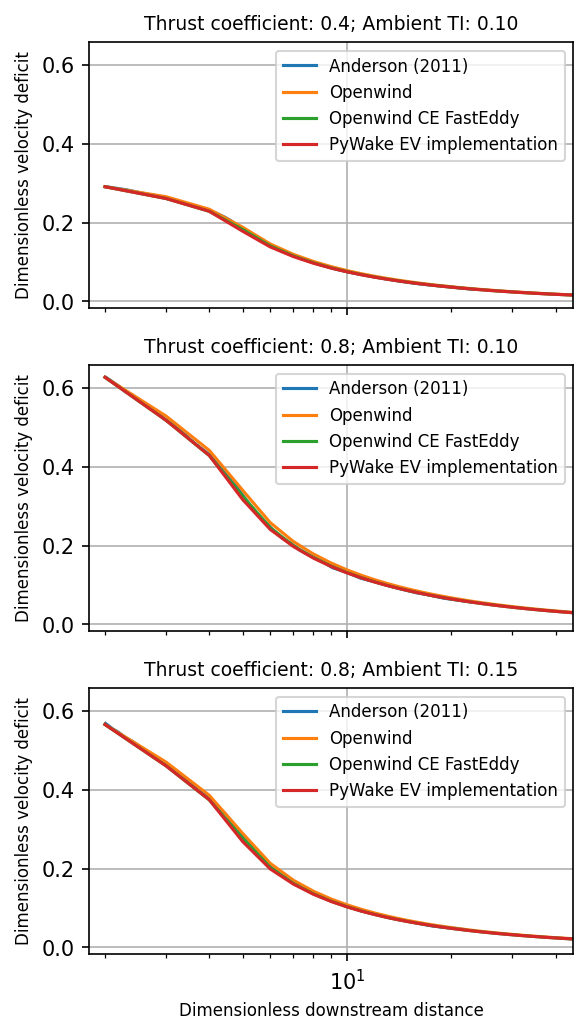
\includegraphics{wake_recovery_results_comparison_mixing_function.png}
	\caption{Comparison of single wake centreline deficit results when the near wake mixing filter function is enabled.}
	\label{fig:wake_recovery_results_comparison_mixing_function}
\end{figure}

A comparison of results for the model configuration without the near wake mixing filter function is presented in Figure \ref{fig:wake_recovery_results_comparison_no_mixing_function}. \textcite{Anderson_2011} did not present results for this case. The results of the PyWake EV model implementation are in close agreement with the Openwind results. The WindFarmer results differ significantly, likely due to having adopted a modified form of the original model equations. The Openwind Theory Manual \parencite{Openwind_Theory_Manual} noted significant differences in EV model results between Openwind and WindFarmer.

\begin{figure}
	\centering
		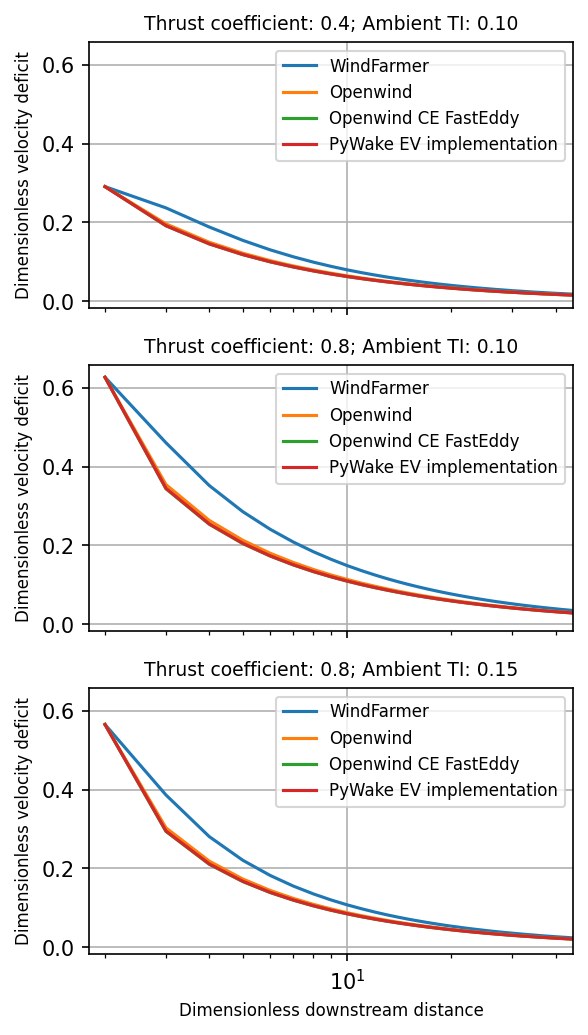
\includegraphics{wake_recovery_results_comparison_no_mixing_function.png}
	\caption{Comparison of single wake centreline deficit results when the near wake mixing filter function is disabled.}
	\label{fig:wake_recovery_results_comparison_no_mixing_function}
\end{figure}

\printbibliography

\end{document}
